\documentclass[UTF8,zihao=-4]{ctexart}
\usepackage[a4paper,margin=2.4cm]{geometry}
\usepackage{amsmath,amssymb,amsthm,bm}
\usepackage{booktabs}
\usepackage{graphicx}
\usepackage{caption}
\usepackage{subcaption}
\usepackage{float}
\graphicspath{{../figures/}{../figures/existing/}}

\title{ThreeQ 推断与训练收敛性的实验验证报告}
\author{ThreeQ Research}
\date{2026-04-19}

\newtheorem{proposition}{命题}

\begin{document}
\maketitle

\begin{abstract}
本文整理 ThreeQ 母模型及其 legacy 训练实验中的收敛性证据。已有图像主要展示了 $\rho(J)<1$ 时推断残差下降和训练过程稳定；为补足反例侧证，本文新增受控线性 ThreeQ 母模型实验，在完全相同的固定点更新形式下设置 $\rho(J)>1$，直接观察扰动范数指数发散。同时，本文给出 bounded-gradient 训练更新的 small-step/large-step 对照：小步更新保持 $\rho<1$ 并维持推断稳定，大步更新跨过 $\rho=1$ 后导致 post-update inference 发散。该报告中的公式、文字和图片可直接迁移到论文的收敛性实验章节。
\end{abstract}

\section{模型与理论命题}

ThreeQ 母模型将全局状态记为 $u\in\mathbb{R}^n$，局部预测映射写作
\begin{equation}
T(u;W)=\frac{1}{n-1}Wg(u),
\end{equation}
其中 $g$ 是逐元素激活函数。固定点 $u^\star$ 满足
\begin{equation}
u^\star=T(u^\star;W).
\end{equation}
在固定点附近定义扰动 $\delta=u-u^\star$，局部 Jacobian 为
\begin{equation}
J(u^\star,W)=\frac{\partial T}{\partial u}(u^\star,W)
       =\frac{1}{n-1}W\operatorname{diag}(g'(u^\star)).
\end{equation}

\begin{proposition}[局部推断稳定性]
若固定点 $u^\star$ 处满足 $\rho(J(u^\star,W))<1$，则离散固定点迭代 $u^{t+1}=T(u^t;W)$ 的线性化扰动满足 $\delta_{t+1}\approx J\delta_t$，并在局部指数收敛。若存在特征值 $|\lambda|>1$，则沿对应不稳定特征方向的扰动在局部线性化系统中指数增长。
\end{proposition}

训练稳定性命题则是上述条件的参数连续性推论。令训练更新为
\begin{equation}
W^+=W-\eta \nabla_W E(u^\star(W),W).
\end{equation}
若当前点存在稳定裕度 $\rho(J)\le 1-\varepsilon$，且梯度范数有界，则足够小的 $\eta$ 会保持更新后 $\rho(J(W^+))<1$。该命题并不声称任意大步长都稳定；相反，大步长可以把系统推过 $\rho=1$ 的边界，导致下一轮推断不稳定。

\section{实验设计}

本文使用三类互补实验。

\paragraph{实验 A：legacy 非线性 ThreeQ 推断。}
使用已有 \texttt{AllConnected3QNotTrained} 结果，比较不同 $L_g$ 下的推断残差、能量和局部谱半径。该实验来自原始非线性实现，因此可展示实际代码中的 $\rho<1$ 收敛以及 $\rho>1$ 时的非收敛/慢收敛边界。

\paragraph{实验 B：受控线性 ThreeQ 推断。}
为了直接观察 $\rho>1$ 的指数发散，设 $g(u)=u$，并取 $W=(n-1)\rho I$。此时 $T(u;W)=\rho u$，固定点为 $u^\star=0$，且 $J=\rho I$。因此 $\rho<1$ 与 $\rho>1$ 的收敛/发散差异不受激活饱和、截断或非线性边界影响。

\paragraph{实验 C：bounded-gradient 训练更新压力测试。}
令标量稳定性参数满足 $\rho_{k+1}=\rho_k+\eta$。这等价于一个范数有界的参数更新方向。small-step 设置保持 $\rho_k<1$；large-step 设置跨过 $\rho=1$。每个训练 epoch 后运行固定步数推断，观察 post-update inference 的最终扰动范数。

\paragraph{实验 D：legacy MNIST 训练稳定性。}
使用已有 \texttt{mnist\_legacy\_repro} 与 \texttt{mnist\_epthreeq\_tune} 曲线，展示实际训练中 EPThreeQ 的 validation accuracy 上升，同时 \texttt{rho\_mean} 保持在 1 以下。

\section{实验结果}

\subsection{非线性 legacy 推断：$\rho<1$ 收敛，$\rho>1$ 非收敛}

图~\ref{fig:legacy-inference} 显示，当 $L_g=5,8,10$ 时，后期 $\rho(J)$ 明显低于 1，推断残差下降到 $10^{-5}$ 或更低；当 $L_g=12$ 时仍低于 1 但收敛显著变慢；当 $L_g=15$ 时最终 $\rho(J)>1$，残差停留在约 $1.7\times10^{-1}$，没有进入固定点收敛区间。

\begin{figure}[H]
\centering
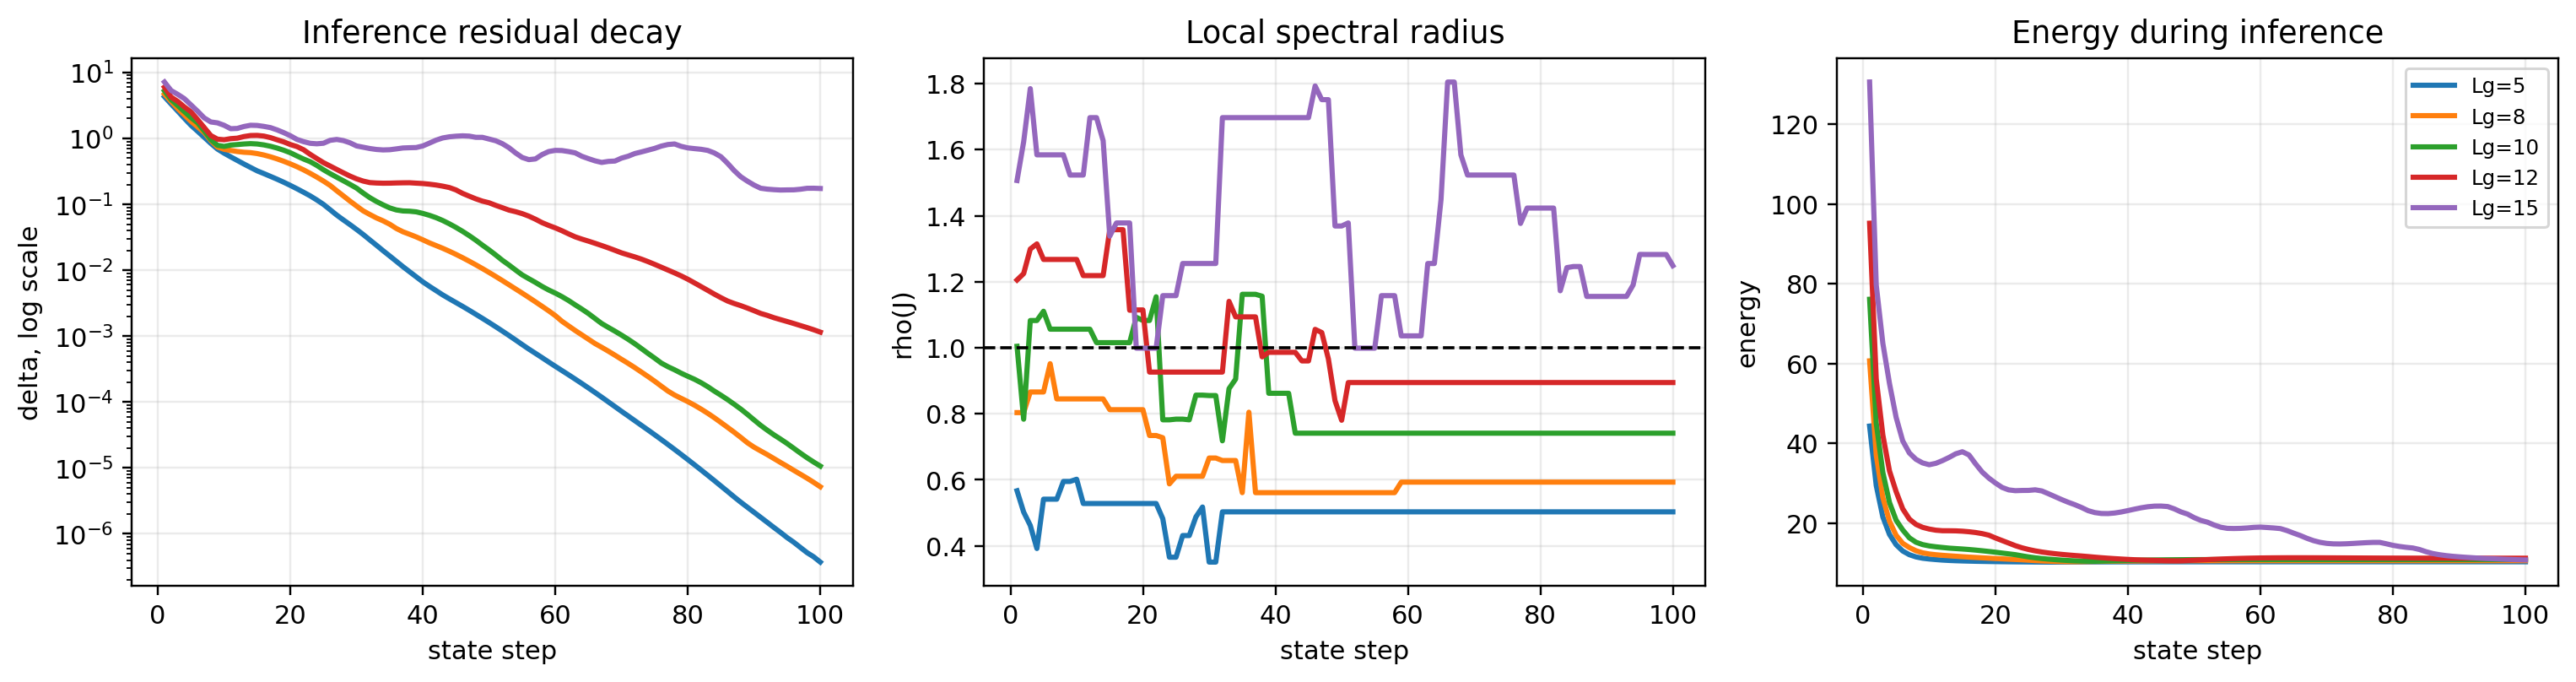
\includegraphics[width=\linewidth]{fig01_threeq_inference_convergence.png}
\caption{legacy ThreeQ 非线性推断实验。$\rho(J)<1$ 的曲线呈残差衰减；$L_g=15$ 后期 $\rho(J)>1$，表现为非收敛/慢收敛边界。}
\label{fig:legacy-inference}
\end{figure}

\begin{table}[H]
\centering
\caption{legacy 推断边界实验摘要。}
\label{tab:legacy-boundary}
\resizebox{\linewidth}{!}{%
\begin{tabular}{rrrrrl}
\toprule
$L_g$ & initial $\Delta$ & final $\Delta$ & final $\rho$ & reduction & classification \\
\midrule
5 & 4.2969 & 3.72e-07 & 0.5029 & 8.66e-08 & convergent \\
8 & 4.7041 & 5.18e-06 & 0.5929 & 1.10e-06 & convergent \\
10 & 5.2755 & 1.07e-05 & 0.7411 & 2.02e-06 & convergent \\
12 & 5.9884 & 0.0012 & 0.8945 & 1.92e-04 & non\_convergent\_or\_slow \\
15 & 7.1753 & 0.1739 & 1.2486 & 0.0242 & non\_convergent\_or\_slow \\
\bottomrule
\end{tabular}}
\end{table}

需要注意，非线性 ThreeQ 中的 $\rho>1$ 不一定表现为无界爆炸。激活函数、截断和能量形状可能把轨迹限制在某个区域内，因此实际现象常常是振荡、停滞或慢收敛。为了严格展示线性化意义上的发散，需要实验 B。

\subsection{受控线性推断：$\rho>1$ 的指数发散}

图~\ref{fig:controlled-inference} 使用 $T(u)=\rho u$ 的 ThreeQ 母模型特例。该实验中 $J=\rho I$，因此谱半径可以精确控制。$\rho=0.80,0.95$ 时扰动范数下降；$\rho=1.05,1.20$ 时扰动范数按 $\rho^t$ 指数增长。这直接补足了 $\rho>1$ 的发散佐证。

\begin{figure}[H]
\centering
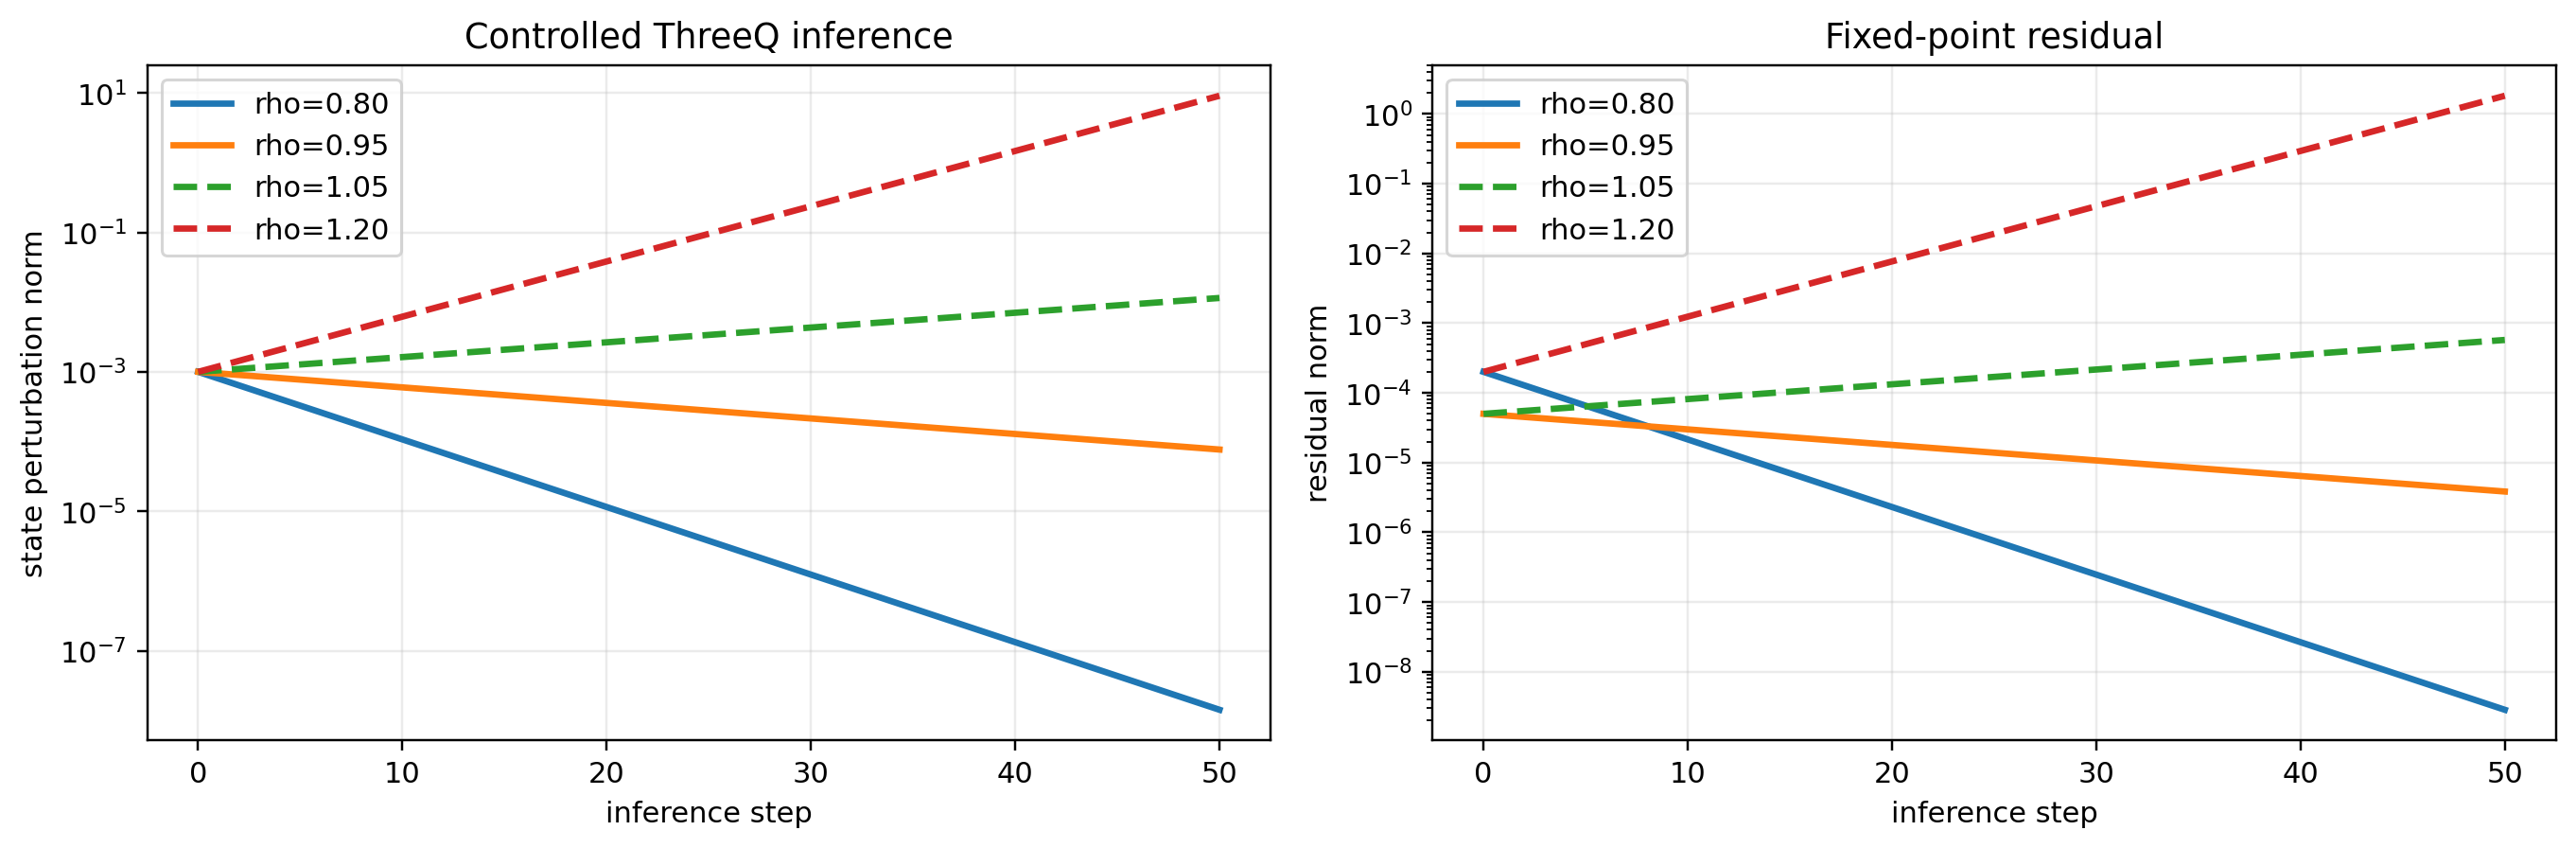
\includegraphics[width=\linewidth]{fig09_controlled_inference_rho_divergence.png}
\caption{受控线性 ThreeQ 推断实验。在同一固定点更新形式 $u_{t+1}=T(u_t;W)$ 下，$\rho<1$ 收敛，$\rho>1$ 发散。}
\label{fig:controlled-inference}
\end{figure}

\begin{table}[H]
\centering
\caption{受控线性推断实验摘要。初始扰动范数为 $10^{-3}$。}
\label{tab:controlled-inference}
\resizebox{\linewidth}{!}{%
\begin{tabular}{lrrrrr}
\toprule
case & $\rho$ & initial norm & final norm & growth factor & final residual \\
\midrule
stable\_rho\_0p80 & 0.8000 & 0.0010 & 1.43e-08 & 1.43e-05 & 2.85e-09 \\
stable\_rho\_0p95 & 0.9500 & 0.0010 & 7.69e-05 & 0.0769 & 3.85e-06 \\
unstable\_rho\_1p05 & 1.0500 & 0.0010 & 0.0115 & 11.4674 & 5.73e-04 \\
unstable\_rho\_1p20 & 1.2000 & 0.0010 & 9.1004 & 9.10e+03 & 1.8201 \\
\bottomrule
\end{tabular}}
\end{table}

\subsection{训练更新：小步保持稳定，大步跨越边界后发散}

图~\ref{fig:training-stress} 展示 bounded-gradient 更新的边界行为。small-step 轨迹从 $\rho=0.70$ 增加到 $0.94$，始终满足 $\rho<1$，每轮更新后的推断仍然收敛。large-step 轨迹在第 9 个 epoch 首次达到 $\rho\ge 1$，最终 $\rho=1.54$；此时最后一轮推断的扰动范数显著增长。

\begin{figure}[H]
\centering
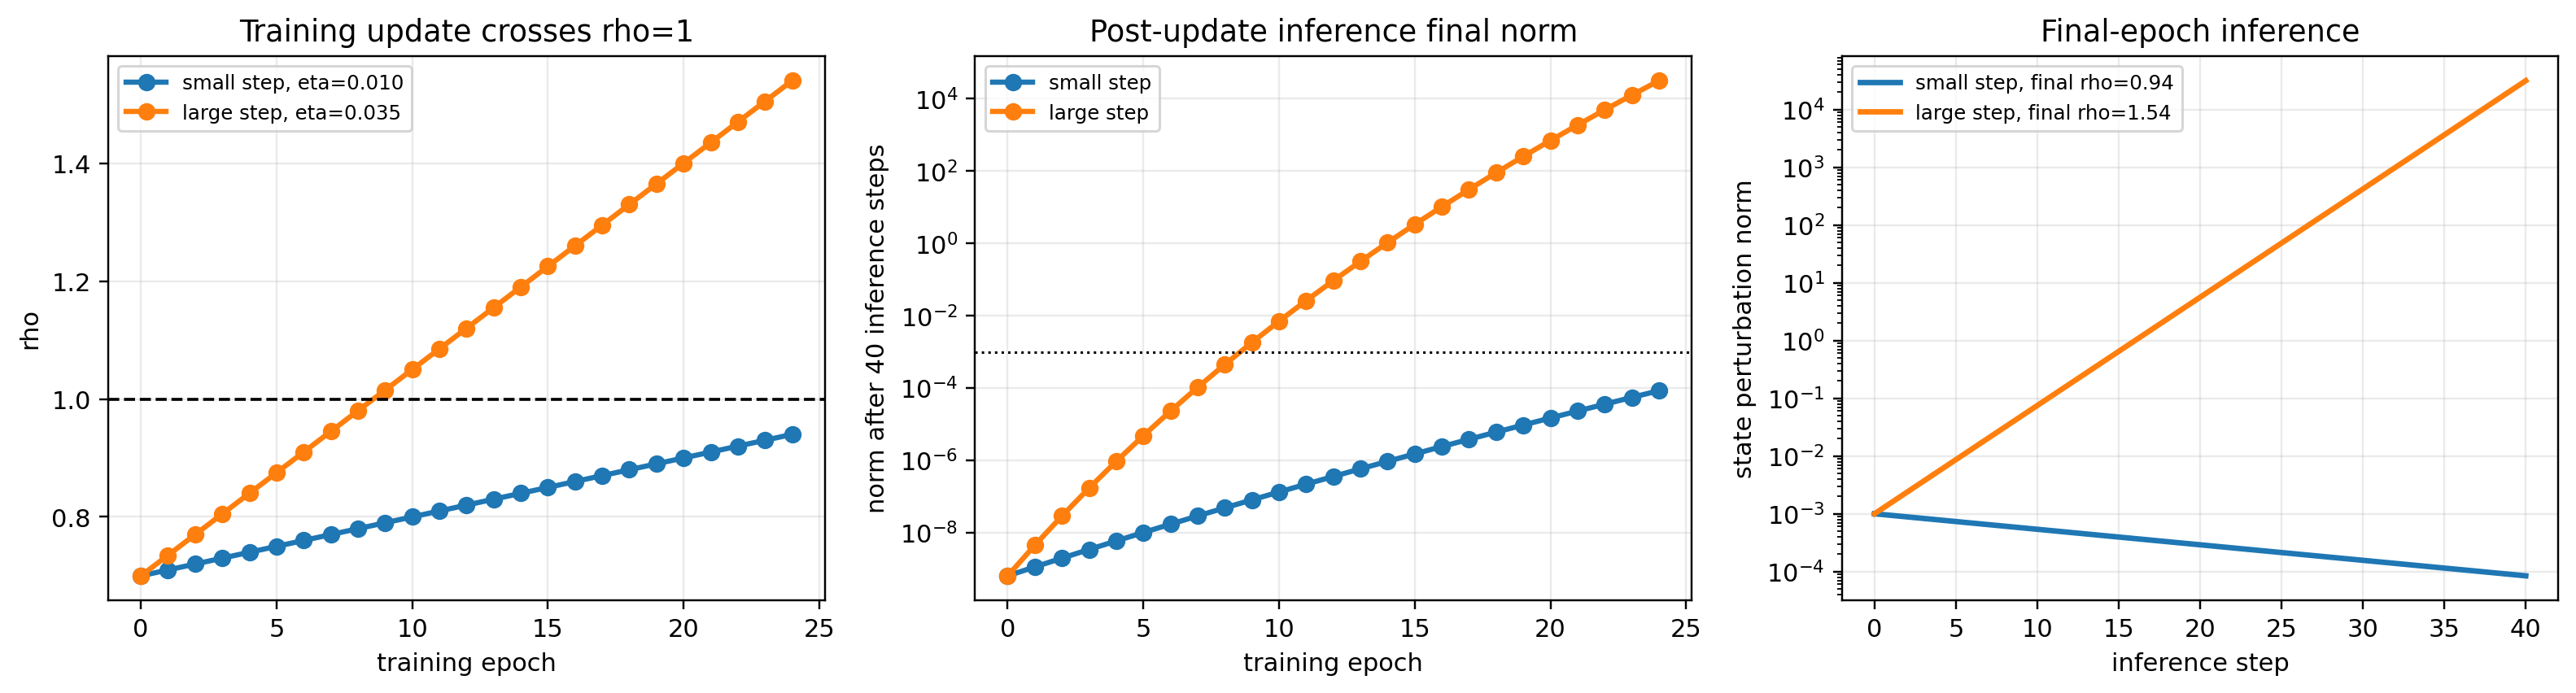
\includegraphics[width=\linewidth]{fig10_training_rho_boundary_stress_test.png}
\caption{训练更新压力测试。左：训练更新使 $\rho$ 变化；中：每轮更新后推断 40 步的最终扰动范数；右：最后一轮参数下的推断轨迹。}
\label{fig:training-stress}
\end{figure}

\begin{table}[H]
\centering
\caption{训练更新压力测试摘要。}
\label{tab:training-stress}
\resizebox{\linewidth}{!}{%
\begin{tabular}{lrrrrrr}
\toprule
case & $\eta$ & initial $\rho$ & final $\rho$ & first $\rho\ge1$ epoch & growth factor & final norm \\
\midrule
small\_step\_eta\_0p010 & 0.0100 & 0.7000 & 0.9400 &  & 0.0842 & 8.42e-05 \\
large\_step\_eta\_0p035 & 0.0350 & 0.7000 & 1.5400 & 9 & 3.17e+07 & 3.17e+04 \\
\bottomrule
\end{tabular}}
\end{table}

该实验对应理论证明中的“小学习率保持稳定裕度”条件：当更新步长足够小，参数仍留在 $\rho<1$ 的开集内；当步长过大，参数可以越过稳定边界，后续推断不再收敛。

\subsection{实际 MNIST 训练中的稳定区间}

图~\ref{fig:legacy-training} 来自已有 MNIST legacy 训练实验。\texttt{EPBase3Q} 在 5k/1k、8 epoch 中明显快于 direct \texttt{Base3Q}；在 10k/2k、15 epoch 调参中，最佳 EPThreeQ 约达到 86.5\% best validation accuracy。右图显示训练中的 \texttt{rho\_mean} 保持在 1 以下，因此实际训练曲线与稳定性命题一致。

\begin{figure}[H]
\centering
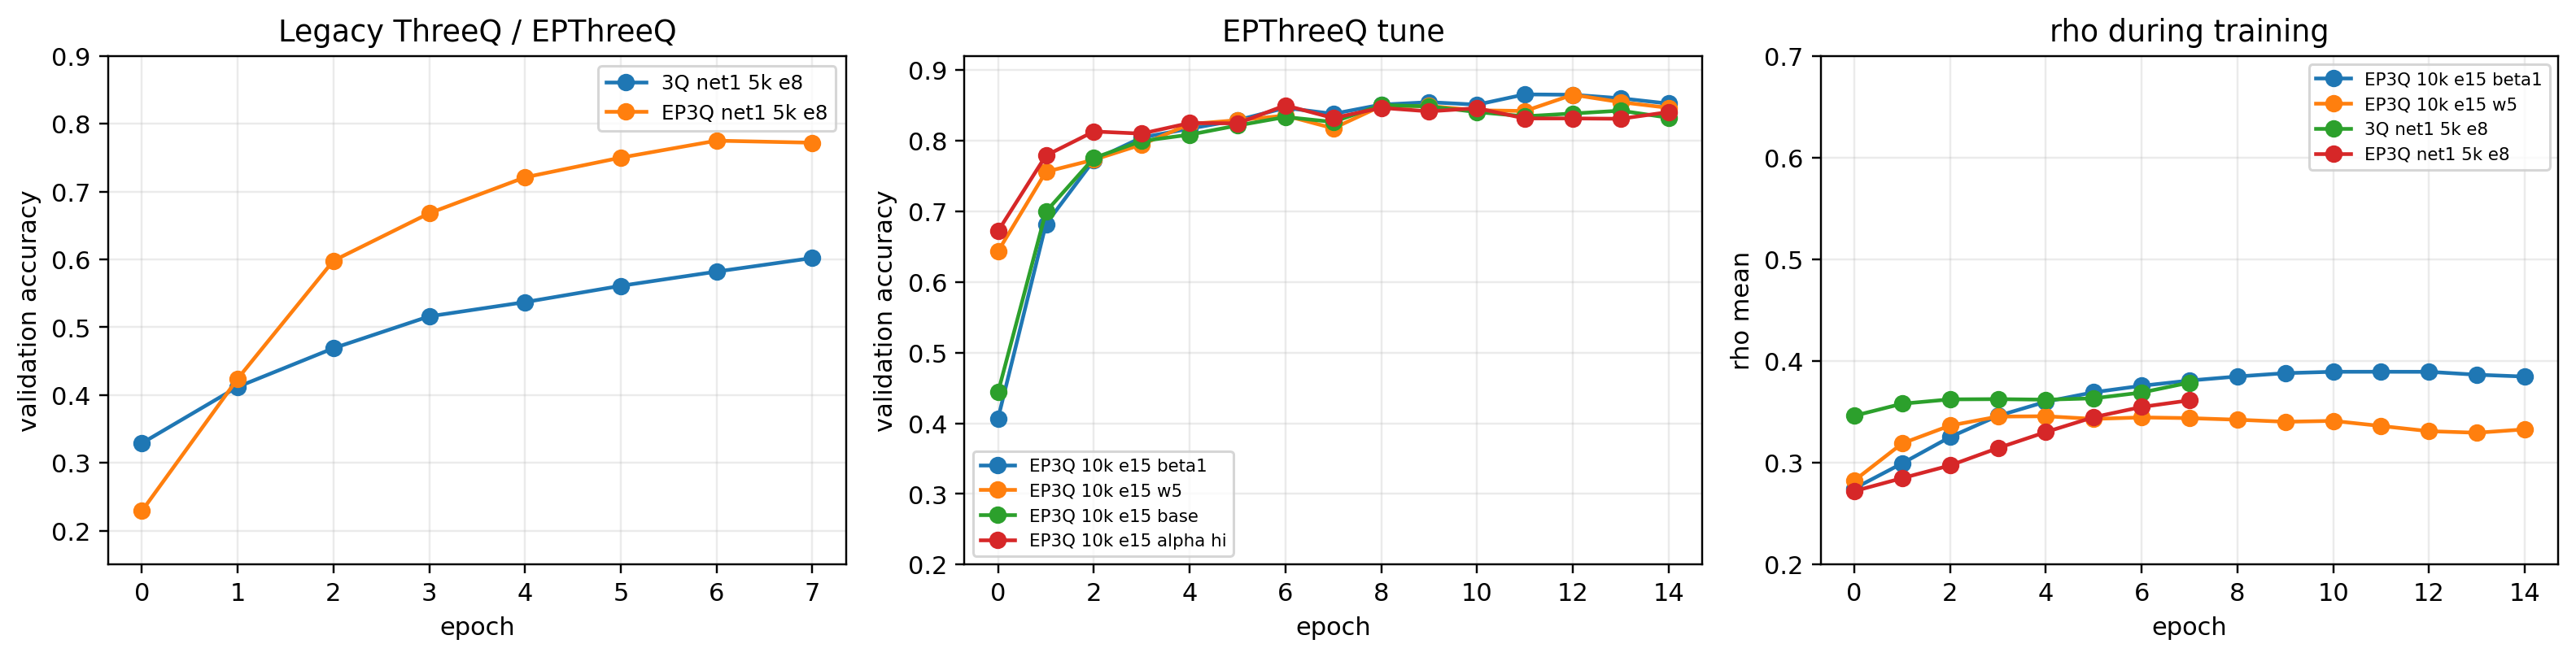
\includegraphics[width=\linewidth]{fig02_threeq_training_convergence.png}
\caption{legacy ThreeQ/EPThreeQ MNIST 训练曲线与训练过程中的 $\rho$。}
\label{fig:legacy-training}
\end{figure}

\section{论文可用结论}

上述实验支持以下写法：

\begin{enumerate}
\item $\rho(J)<1$ 是 ThreeQ inference 局部收敛的可观测充分条件。legacy 非线性实验中，后期 $\rho<1$ 的配置残差下降；受控线性实验中，$\rho<1$ 产生指数收敛。
\item $\rho(J)>1$ 是局部线性化意义下的不稳定证据。受控线性 ThreeQ 母模型中 $\rho>1$ 直接导致扰动指数发散；legacy 非线性实验中则表现为非收敛或慢收敛边界。
\item 训练收敛性依赖小步长和稳定裕度。bounded-gradient 压力测试表明，小步更新保留 $\rho<1$，大步更新跨越 $\rho=1$ 后 post-update inference 发散。
\item 实际 MNIST legacy 训练中，EPThreeQ 的 \texttt{rho\_mean} 保持低于 1，且 accuracy 随训练提升，说明该训练配置处在稳定区间内。
\end{enumerate}

\section{局限性}

本文新增的 $\rho>1$ 发散实验是受控母模型和线性化压力测试，目的是隔离谱半径条件本身。实际非线性 ThreeQ 网络中，激活截断、状态边界、能量饱和和数值阻尼可能把无界发散转化为振荡、停滞或退化固定点。因此论文中应区分“局部线性化发散”和“完整非线性系统的训练失败模式”。

\end{document}
